% Options for packages loaded elsewhere
\PassOptionsToPackage{unicode}{hyperref}
\PassOptionsToPackage{hyphens}{url}
\PassOptionsToPackage{dvipsnames,svgnames,x11names}{xcolor}
%
\documentclass[
  letterpaper,
  DIV=11,
  numbers=noendperiod]{scrartcl}

\usepackage{amsmath,amssymb}
\usepackage{iftex}
\ifPDFTeX
  \usepackage[T1]{fontenc}
  \usepackage[utf8]{inputenc}
  \usepackage{textcomp} % provide euro and other symbols
\else % if luatex or xetex
  \usepackage{unicode-math}
  \defaultfontfeatures{Scale=MatchLowercase}
  \defaultfontfeatures[\rmfamily]{Ligatures=TeX,Scale=1}
\fi
\usepackage{lmodern}
\ifPDFTeX\else  
    % xetex/luatex font selection
\fi
% Use upquote if available, for straight quotes in verbatim environments
\IfFileExists{upquote.sty}{\usepackage{upquote}}{}
\IfFileExists{microtype.sty}{% use microtype if available
  \usepackage[]{microtype}
  \UseMicrotypeSet[protrusion]{basicmath} % disable protrusion for tt fonts
}{}
\makeatletter
\@ifundefined{KOMAClassName}{% if non-KOMA class
  \IfFileExists{parskip.sty}{%
    \usepackage{parskip}
  }{% else
    \setlength{\parindent}{0pt}
    \setlength{\parskip}{6pt plus 2pt minus 1pt}}
}{% if KOMA class
  \KOMAoptions{parskip=half}}
\makeatother
\usepackage{xcolor}
\setlength{\emergencystretch}{3em} % prevent overfull lines
\setcounter{secnumdepth}{-\maxdimen} % remove section numbering
% Make \paragraph and \subparagraph free-standing
\ifx\paragraph\undefined\else
  \let\oldparagraph\paragraph
  \renewcommand{\paragraph}[1]{\oldparagraph{#1}\mbox{}}
\fi
\ifx\subparagraph\undefined\else
  \let\oldsubparagraph\subparagraph
  \renewcommand{\subparagraph}[1]{\oldsubparagraph{#1}\mbox{}}
\fi


\providecommand{\tightlist}{%
  \setlength{\itemsep}{0pt}\setlength{\parskip}{0pt}}\usepackage{longtable,booktabs,array}
\usepackage{calc} % for calculating minipage widths
% Correct order of tables after \paragraph or \subparagraph
\usepackage{etoolbox}
\makeatletter
\patchcmd\longtable{\par}{\if@noskipsec\mbox{}\fi\par}{}{}
\makeatother
% Allow footnotes in longtable head/foot
\IfFileExists{footnotehyper.sty}{\usepackage{footnotehyper}}{\usepackage{footnote}}
\makesavenoteenv{longtable}
\usepackage{graphicx}
\makeatletter
\def\maxwidth{\ifdim\Gin@nat@width>\linewidth\linewidth\else\Gin@nat@width\fi}
\def\maxheight{\ifdim\Gin@nat@height>\textheight\textheight\else\Gin@nat@height\fi}
\makeatother
% Scale images if necessary, so that they will not overflow the page
% margins by default, and it is still possible to overwrite the defaults
% using explicit options in \includegraphics[width, height, ...]{}
\setkeys{Gin}{width=\maxwidth,height=\maxheight,keepaspectratio}
% Set default figure placement to htbp
\makeatletter
\def\fps@figure{htbp}
\makeatother
% definitions for citeproc citations
\NewDocumentCommand\citeproctext{}{}
\NewDocumentCommand\citeproc{mm}{%
  \begingroup\def\citeproctext{#2}\cite{#1}\endgroup}
\makeatletter
 % allow citations to break across lines
 \let\@cite@ofmt\@firstofone
 % avoid brackets around text for \cite:
 \def\@biblabel#1{}
 \def\@cite#1#2{{#1\if@tempswa , #2\fi}}
\makeatother
\newlength{\cslhangindent}
\setlength{\cslhangindent}{1.5em}
\newlength{\csllabelwidth}
\setlength{\csllabelwidth}{3em}
\newenvironment{CSLReferences}[2] % #1 hanging-indent, #2 entry-spacing
 {\begin{list}{}{%
  \setlength{\itemindent}{0pt}
  \setlength{\leftmargin}{0pt}
  \setlength{\parsep}{0pt}
  % turn on hanging indent if param 1 is 1
  \ifodd #1
   \setlength{\leftmargin}{\cslhangindent}
   \setlength{\itemindent}{-1\cslhangindent}
  \fi
  % set entry spacing
  \setlength{\itemsep}{#2\baselineskip}}}
 {\end{list}}
\usepackage{calc}
\newcommand{\CSLBlock}[1]{\hfill\break\parbox[t]{\linewidth}{\strut\ignorespaces#1\strut}}
\newcommand{\CSLLeftMargin}[1]{\parbox[t]{\csllabelwidth}{\strut#1\strut}}
\newcommand{\CSLRightInline}[1]{\parbox[t]{\linewidth - \csllabelwidth}{\strut#1\strut}}
\newcommand{\CSLIndent}[1]{\hspace{\cslhangindent}#1}

\KOMAoption{captions}{tableheading}
\makeatletter
\@ifpackageloaded{caption}{}{\usepackage{caption}}
\AtBeginDocument{%
\ifdefined\contentsname
  \renewcommand*\contentsname{Table of contents}
\else
  \newcommand\contentsname{Table of contents}
\fi
\ifdefined\listfigurename
  \renewcommand*\listfigurename{List of Figures}
\else
  \newcommand\listfigurename{List of Figures}
\fi
\ifdefined\listtablename
  \renewcommand*\listtablename{List of Tables}
\else
  \newcommand\listtablename{List of Tables}
\fi
\ifdefined\figurename
  \renewcommand*\figurename{Figure}
\else
  \newcommand\figurename{Figure}
\fi
\ifdefined\tablename
  \renewcommand*\tablename{Table}
\else
  \newcommand\tablename{Table}
\fi
}
\@ifpackageloaded{float}{}{\usepackage{float}}
\floatstyle{ruled}
\@ifundefined{c@chapter}{\newfloat{codelisting}{h}{lop}}{\newfloat{codelisting}{h}{lop}[chapter]}
\floatname{codelisting}{Listing}
\newcommand*\listoflistings{\listof{codelisting}{List of Listings}}
\makeatother
\makeatletter
\makeatother
\makeatletter
\@ifpackageloaded{caption}{}{\usepackage{caption}}
\@ifpackageloaded{subcaption}{}{\usepackage{subcaption}}
\makeatother
\ifLuaTeX
  \usepackage{selnolig}  % disable illegal ligatures
\fi
\usepackage{bookmark}

\IfFileExists{xurl.sty}{\usepackage{xurl}}{} % add URL line breaks if available
\urlstyle{same} % disable monospaced font for URLs
\hypersetup{
  pdftitle={Stellar Classification using Photometric data},
  pdfauthor={Olivia Lam, Aron Braham, Lucy Liu, and Viet Ngo},
  colorlinks=true,
  linkcolor={blue},
  filecolor={Maroon},
  citecolor={Blue},
  urlcolor={Blue},
  pdfcreator={LaTeX via pandoc}}

\title{Stellar Classification using Photometric data}
\author{Olivia Lam, Aron Braham, Lucy Liu, and Viet Ngo}
\date{}

\begin{document}
\maketitle

\renewcommand*\contentsname{Table of contents}
{
\hypersetup{linkcolor=}
\setcounter{tocdepth}{2}
\tableofcontents
}
\subsection{Summary}\label{summary}

In this report, we attempt to build a classification model using
logistic regression which uses photo metric measurements from telescopes
to classify stars under the Morgan-Keenan system. Our final classifier
performed poorly with a low accuracy on testing data set with a tendency
to classify stars as one class cooler than its actual class type. Our
model can only classify stars into four main classes due to the small
sample size. It is recommended that further study using larger sample
sizes and methods to improve the classification model.

\subsection{Introduction}\label{introduction}

Current and future astronomical surveys will observe hundred of
thousands of objects each year. Due to the massive amount of
spectroscopic and photometric data produced, an automated stellar
classification process has become important in the field of astronomy in
the past few years.

In astronomy, understanding the spectral characteristics of celestial
objects serves as a fundamental pillar for unraveling the mysteries of
the cosmos. Spectral classification, a cornerstone of astronomical
research, enables us to discern the chemical composition, temperature,
and evolutionary stage of stars, galaxies, and other celestial bodies.
In the earliest days it was based on mass and temperature; however, our
modern classification system has evolved and we classify stars based on
the Morgan--Keenan (MK) system (Morgan, Keenan, and Kellman 1942) which
group stars into 7 classes based on their spectral characteristics.
Under the MK system, astronomers analyse electromagnetic radiation from
stars to determine its class. These electromagnetic spectrum have dark
lines to determine which and how abundant elements are present in the
star. The seven classes in the MK system - O, B, A, F, G, K, and M - are
sequenced from the hottest (O type) to the coolest (K type) which also
exhibits a certain characteristic that is very visible - colour. Hence
in this report, we will classify stars using photometric data and in the
Discussion section, we will evaluate whether this is a reliable
alternative for the traditional method of comparing the best fit of the
spectra to that of templates using statistical tests (Duan et al. 2009).

\subsubsection{Definitions}\label{definitions}

\textbf{Photometry}: the measurement of the flux or intensity of an
astronomical object's electromagnetic radiation

The photo metric system we're using to classify star types is the
\emph{Sloan} system (Kent 1994) used by the Sloan Digital Sky Survey.
The system measures the intensity of electromagnetic radition from stars
at 5 bands: - \emph{u} (345nm) - \emph{g} (475nm which is a light blue
in the visible spectrum) - \emph{r} (622nm which is orange) - \emph{i}
(763nm which is deep red) - \emph{z} (905nm)

\subsection{Methods \& Results}\label{methods-results}

\subsubsection{Data}\label{data}

This report has made use of the NASA Exoplanet Archive, which is
operated by the California Institute of Technology, under contract with
the National Aeronautics and Space Administration under the Exoplanet
Exploration Program. NASA Exoplanet Archive collects data from various
sources, including ground-based observatories and space telescopes such
as the Kepler Space Telescope and the Transiting Exoplanet Survey
Satellite (TESS). The dataset is we're using is their
\href{https://exoplanetarchive.ipac.caltech.edu/cgi-bin/TblView/nph-tblView?app=ExoTbls&config=PS}{Planetary
Systems dataset} which has the columns of names, spectral type and
measurements using Sloan photometric system selected.

The Python programming language (Van Rossum and Drake Jr 1995) and the
following Python packages were used to perform the analysis:
\texttt{matplotlib} (Hunter 2007), \texttt{scikit-learn} (Pedregosa et
al. 2011) and \texttt{Pandas} (McKinney et al. 2010).

\subsubsection{Imports}\label{imports}

First of all, let's import the packages we will use to carry out the
analysis and download the dataset. For our analysis we primarily used
\texttt{sklearn} and \texttt{pandas} for our classification analysis as
well as \texttt{matplotlib} for our visualizations.

\subsubsection{Reading the Dataset}\label{reading-the-dataset}

We then download the dataset of interest: the Expoplanet Systems dataset
from NASA, containing information about measurements of planets and
stars. We are interested in the spectral type of stars given a subset of
these measurements.

\begin{longtable}[]{@{}
  >{\raggedright\arraybackslash}p{(\columnwidth - 12\tabcolsep) * \real{0.1414}}
  >{\raggedright\arraybackslash}p{(\columnwidth - 12\tabcolsep) * \real{0.1515}}
  >{\raggedleft\arraybackslash}p{(\columnwidth - 12\tabcolsep) * \real{0.1414}}
  >{\raggedleft\arraybackslash}p{(\columnwidth - 12\tabcolsep) * \real{0.1414}}
  >{\raggedleft\arraybackslash}p{(\columnwidth - 12\tabcolsep) * \real{0.1414}}
  >{\raggedleft\arraybackslash}p{(\columnwidth - 12\tabcolsep) * \real{0.1414}}
  >{\raggedleft\arraybackslash}p{(\columnwidth - 12\tabcolsep) * \real{0.1414}}@{}}

\caption{\label{tbl-read-data}Table of our Initial Data}

\tabularnewline

\toprule\noalign{}
\begin{minipage}[b]{\linewidth}\raggedright
pl\_name
\end{minipage} & \begin{minipage}[b]{\linewidth}\raggedright
st\_spectype
\end{minipage} & \begin{minipage}[b]{\linewidth}\raggedleft
sy\_umagstr
\end{minipage} & \begin{minipage}[b]{\linewidth}\raggedleft
sy\_gmagstr
\end{minipage} & \begin{minipage}[b]{\linewidth}\raggedleft
sy\_rmagstr
\end{minipage} & \begin{minipage}[b]{\linewidth}\raggedleft
sy\_imagstr
\end{minipage} & \begin{minipage}[b]{\linewidth}\raggedleft
sy\_zmagstr
\end{minipage} \\
\midrule\noalign{}
\endhead
\bottomrule\noalign{}
\endlastfoot
OGLE-TR-10 b & nan & nan & nan & nan & nan & nan \\
BD-08 2823 b & K3 V & nan & nan & nan & nan & nan \\
BD-08 2823 c & K3 V & nan & nan & nan & nan & nan \\
HR 8799 c & A5 V & nan & nan & nan & nan & nan \\
HD 104985 b & nan & nan & nan & nan & nan & nan \\
4 UMa b & K1 III & nan & nan & nan & nan & nan \\
HD 104985 b & G9 III & nan & nan & nan & nan & nan \\
kap CrB b & nan & nan & nan & nan & nan & nan \\
kap CrB b & nan & nan & nan & nan & nan & nan \\
kap CrB b & nan & nan & nan & nan & nan & nan \\

\end{longtable}

\subsection{Data EDA and Wrangling}\label{data-eda-and-wrangling}

This dataset from NASA's Exoplanet Archive include all planets and
stars. Therefore we will wrangle the dataset such that it only contain
stars with Sloan magnitudes for photometric measurements.

Below in Table~\ref{tbl-cleaned-data} our preprocessing included
dropping NA values from our \texttt{spec\_type} and band star brightness
features. We are also only interested in the first letter of the
spectral type, which becomes our y value later in the analysis, so we
modified that feature as well.

\begin{longtable}[]{@{}
  >{\raggedright\arraybackslash}p{(\columnwidth - 12\tabcolsep) * \real{0.1667}}
  >{\raggedright\arraybackslash}p{(\columnwidth - 12\tabcolsep) * \real{0.1786}}
  >{\raggedleft\arraybackslash}p{(\columnwidth - 12\tabcolsep) * \real{0.1310}}
  >{\raggedleft\arraybackslash}p{(\columnwidth - 12\tabcolsep) * \real{0.1310}}
  >{\raggedleft\arraybackslash}p{(\columnwidth - 12\tabcolsep) * \real{0.1310}}
  >{\raggedleft\arraybackslash}p{(\columnwidth - 12\tabcolsep) * \real{0.1310}}
  >{\raggedleft\arraybackslash}p{(\columnwidth - 12\tabcolsep) * \real{0.1310}}@{}}

\caption{\label{tbl-cleaned-data}Table of our Cleaned Dataset}

\tabularnewline

\toprule\noalign{}
\begin{minipage}[b]{\linewidth}\raggedright
pl\_name
\end{minipage} & \begin{minipage}[b]{\linewidth}\raggedright
st\_spectype
\end{minipage} & \begin{minipage}[b]{\linewidth}\raggedleft
sy\_umag
\end{minipage} & \begin{minipage}[b]{\linewidth}\raggedleft
sy\_gmag
\end{minipage} & \begin{minipage}[b]{\linewidth}\raggedleft
sy\_rmag
\end{minipage} & \begin{minipage}[b]{\linewidth}\raggedleft
sy\_imag
\end{minipage} & \begin{minipage}[b]{\linewidth}\raggedleft
sy\_zmag
\end{minipage} \\
\midrule\noalign{}
\endhead
\bottomrule\noalign{}
\endlastfoot
TOI-2084 b & M & 18.6919 & 16.0801 & 14.6494 & 17.9112 & 13.2406 \\
TOI-1801 b & M & 16.4486 & 12.6586 & 11.0055 & 10.2729 & 10.7555 \\
K2-133 c & M & 17.2832 & 15.2645 & 13.6265 & 12.9151 & 12.7195 \\
K2-133 e & M & 17.2832 & 15.2645 & 13.6265 & 12.9151 & 12.7195 \\
K2-133 d & M & 17.2832 & 15.2645 & 13.6265 & 12.9151 & 12.7195 \\
TOI-3785 b & M & 17.9187 & 15.4753 & 14.0744 & 13.2233 & 12.4056 \\
TOI-3984 A b & M & 19.1895 & 16.5597 & 15.1645 & 13.9346 & 13.2853 \\
TOI-1853 b & K & 15.5075 & 14.9806 & 11.9848 & 11.7529 & 11.8545 \\
Wolf 327 b & M & 16.6342 & 15.6776 & 14.839 & 14.9466 & 11.0601 \\
HD 81688 b & K & 13.0932 & 10.9213 & 9.31906 & 8.71834 & 7.85169 \\

\end{longtable}

\textbf{Note}: In order to run classification models on our dataset, we
had to remove the NA values from our magnitudes. We were planning to
incorporate \texttt{SimpleImputer()} into our pipeline during data
preprocessing, but about 2200 rows contained NA values, so we thought it
was best to simply drop them. This explains the drastic decrease in
observations.

\subsubsection{Variable Descriptions:}\label{variable-descriptions}

\texttt{st\_spectype}: Classification of the star based on their
spectral characteristics following the Morgan-Keenan system

\texttt{sy\_umag}: Brightness of the host star as measured using the
Sloan Digital Sky Survey (SDSS) u band, in units of magnitudes

\texttt{sy\_gmag}: Brightness of the host star as measured using the
Sloan Digital Sky Survey (SDSS) g band, in units of magnitudes

\texttt{sy\_rmag}: Brightness of the host star as measured using the
Sloan Digital Sky Survey (SDSS) r band, in units of magnitudes

\texttt{sy\_imag}: Brightness of the host star as measured using the
Sloan Digital Sky Survey (SDSS) i band, in units of magnitudes

\texttt{sy\_zmag}: Brightness of the host star as measured using the
Sloan Digital Sky Survey (SDSS) z band, in units of magnitudes

From our Figure~\ref{fig-sy-umag} visualization below we can see that
our highest stellar value counts was for the \emph{M} class, followed
respectively by \emph{K}, \emph{G}, and \emph{F}.

\begin{figure}[H]

\centering{

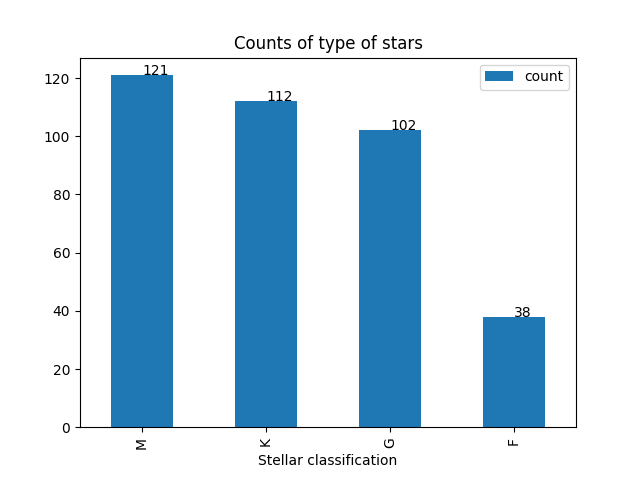
\includegraphics[width=0.9\textwidth,height=\textheight]{../results/figures/star_count_hist.png}

}

\caption{\label{fig-sy-umag}\texttt{Histogram\ of\ Star\ Count\ Values}}

\end{figure}%

Now we will explore the features and boxplots of each band's magnitude
for our four types of stellar classifications.

\begin{longtable}[]{@{}
  >{\raggedright\arraybackslash}p{(\columnwidth - 16\tabcolsep) * \real{0.1022}}
  >{\raggedright\arraybackslash}p{(\columnwidth - 16\tabcolsep) * \real{0.0803}}
  >{\raggedright\arraybackslash}p{(\columnwidth - 16\tabcolsep) * \real{0.1460}}
  >{\raggedright\arraybackslash}p{(\columnwidth - 16\tabcolsep) * \real{0.1460}}
  >{\raggedright\arraybackslash}p{(\columnwidth - 16\tabcolsep) * \real{0.0949}}
  >{\raggedright\arraybackslash}p{(\columnwidth - 16\tabcolsep) * \real{0.1460}}
  >{\raggedright\arraybackslash}p{(\columnwidth - 16\tabcolsep) * \real{0.0949}}
  >{\raggedright\arraybackslash}p{(\columnwidth - 16\tabcolsep) * \real{0.0949}}
  >{\raggedright\arraybackslash}p{(\columnwidth - 16\tabcolsep) * \real{0.0949}}@{}}

\caption{\label{tbl-sy-umag}Table of sy\_umag Features}

\tabularnewline

\toprule\noalign{}
\begin{minipage}[b]{\linewidth}\raggedright
Unnamed: 0
\end{minipage} & \begin{minipage}[b]{\linewidth}\raggedright
sy\_umag
\end{minipage} & \begin{minipage}[b]{\linewidth}\raggedright
sy\_umag.1
\end{minipage} & \begin{minipage}[b]{\linewidth}\raggedright
sy\_umag.2
\end{minipage} & \begin{minipage}[b]{\linewidth}\raggedright
sy\_umag.3
\end{minipage} & \begin{minipage}[b]{\linewidth}\raggedright
sy\_umag.4
\end{minipage} & \begin{minipage}[b]{\linewidth}\raggedright
sy\_umag.5
\end{minipage} & \begin{minipage}[b]{\linewidth}\raggedright
sy\_umag.6
\end{minipage} & \begin{minipage}[b]{\linewidth}\raggedright
sy\_umag.7
\end{minipage} \\
\midrule\noalign{}
\endhead
\bottomrule\noalign{}
\endlastfoot
nan & count & mean & std & min & 25\% & 50\% & 75\% & max \\
st\_spectype & nan & nan & nan & nan & nan & nan & nan & nan \\
F & 38.0 & 15.006642105263154 & 0.766401328650734 & 13.7542 & 14.7063 &
14.8961 & 15.2332 & 17.9494 \\
G & 102.0 & 15.184445098039218 & 0.5159733968557502 & 13.9531 &
15.005849999999999 & 15.166 & 15.4862 & 16.9794 \\
K & 112.0 & 15.60805535714286 & 0.8534817900324461 & 13.0932 & 15.0413 &
15.56765 & 15.8447 & 17.9905 \\
M & 121.0 & 17.467182644628096 & 1.812482452589895 & 14.5112 & 15.7198 &
17.2832 & 19.1895 & 21.2975 \\

\end{longtable}

\begin{figure}[H]

{\centering 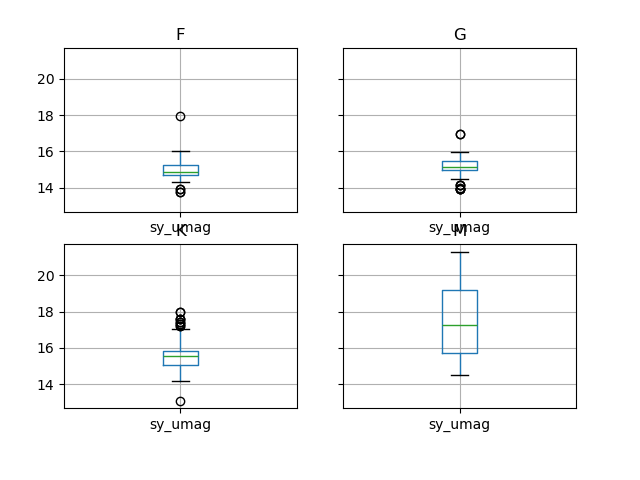
\includegraphics[width=0.9\textwidth,height=\textheight]{../results/figures/sy_umag.png}

}

\caption{Box Plot of \texttt{fig-sy-umag}}

\end{figure}%

From boxplot Figure~\ref{fig-sy-umag}, for \emph{M}-class of stars, the
magnitude of the \emph{u}-band is much higher than the remaining classes
at 17.3 at the median.

\begin{longtable}[]{@{}
  >{\raggedright\arraybackslash}p{(\columnwidth - 16\tabcolsep) * \real{0.1022}}
  >{\raggedright\arraybackslash}p{(\columnwidth - 16\tabcolsep) * \real{0.0803}}
  >{\raggedright\arraybackslash}p{(\columnwidth - 16\tabcolsep) * \real{0.1460}}
  >{\raggedright\arraybackslash}p{(\columnwidth - 16\tabcolsep) * \real{0.1460}}
  >{\raggedright\arraybackslash}p{(\columnwidth - 16\tabcolsep) * \real{0.0949}}
  >{\raggedright\arraybackslash}p{(\columnwidth - 16\tabcolsep) * \real{0.0949}}
  >{\raggedright\arraybackslash}p{(\columnwidth - 16\tabcolsep) * \real{0.1460}}
  >{\raggedright\arraybackslash}p{(\columnwidth - 16\tabcolsep) * \real{0.0949}}
  >{\raggedright\arraybackslash}p{(\columnwidth - 16\tabcolsep) * \real{0.0949}}@{}}

\caption{\label{tbl-sy-gmag}Table of sy\_gmag Features}

\tabularnewline

\toprule\noalign{}
\begin{minipage}[b]{\linewidth}\raggedright
Unnamed: 0
\end{minipage} & \begin{minipage}[b]{\linewidth}\raggedright
sy\_gmag
\end{minipage} & \begin{minipage}[b]{\linewidth}\raggedright
sy\_gmag.1
\end{minipage} & \begin{minipage}[b]{\linewidth}\raggedright
sy\_gmag.2
\end{minipage} & \begin{minipage}[b]{\linewidth}\raggedright
sy\_gmag.3
\end{minipage} & \begin{minipage}[b]{\linewidth}\raggedright
sy\_gmag.4
\end{minipage} & \begin{minipage}[b]{\linewidth}\raggedright
sy\_gmag.5
\end{minipage} & \begin{minipage}[b]{\linewidth}\raggedright
sy\_gmag.6
\end{minipage} & \begin{minipage}[b]{\linewidth}\raggedright
sy\_gmag.7
\end{minipage} \\
\midrule\noalign{}
\endhead
\bottomrule\noalign{}
\endlastfoot
nan & count & mean & std & min & 25\% & 50\% & 75\% & max \\
st\_spectype & nan & nan & nan & nan & nan & nan & nan & nan \\
F & 38.0 & 13.40213157894737 & 1.4915812676132458 & 10.7614 & 12.064725
& 13.243500000000001 & 14.971975 & 16.4513 \\
G & 102.0 & 13.375269607843137 & 1.0365262651636484 & 10.4929 & 12.65185
& 13.3064 & 14.1084 & 15.387 \\
K & 112.0 & 13.141451785714285 & 1.7709205577322165 & 10.0139 & 11.3126
& 13.0851 & 14.8948 & 16.0648 \\
M & 121.0 & 14.89958826446281 & 2.0709525814057472 & 9.91288 & 13.021 &
15.3392 & 16.452 & 18.7296 \\

\end{longtable}

\begin{figure}[H]

\centering{

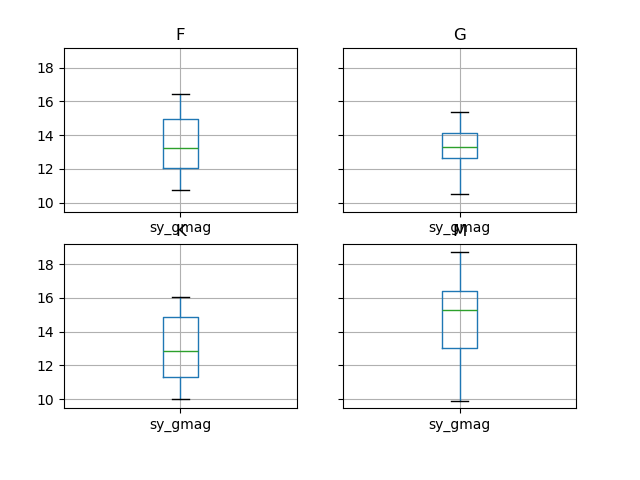
\includegraphics[width=0.9\textwidth,height=\textheight]{../results/figures/sy_gmag.png}

}

\caption{\label{fig-sy-gmag}Box Plot of \texttt{sy\_gmag}}

\end{figure}%

Again, from boxplot Figure~\ref{fig-sy-gmag}, for \emph{M}-class of
stars, the magnitude of the \emph{g}-band is much higher than the
remaining classes at 15.3 at the median.

\begin{longtable}[]{@{}
  >{\raggedright\arraybackslash}p{(\columnwidth - 16\tabcolsep) * \real{0.1022}}
  >{\raggedright\arraybackslash}p{(\columnwidth - 16\tabcolsep) * \real{0.0803}}
  >{\raggedright\arraybackslash}p{(\columnwidth - 16\tabcolsep) * \real{0.1460}}
  >{\raggedright\arraybackslash}p{(\columnwidth - 16\tabcolsep) * \real{0.1460}}
  >{\raggedright\arraybackslash}p{(\columnwidth - 16\tabcolsep) * \real{0.0949}}
  >{\raggedright\arraybackslash}p{(\columnwidth - 16\tabcolsep) * \real{0.0949}}
  >{\raggedright\arraybackslash}p{(\columnwidth - 16\tabcolsep) * \real{0.1460}}
  >{\raggedright\arraybackslash}p{(\columnwidth - 16\tabcolsep) * \real{0.0949}}
  >{\raggedright\arraybackslash}p{(\columnwidth - 16\tabcolsep) * \real{0.0949}}@{}}

\caption{\label{tbl-sy-rmag}Table of sy\_rmag Features}

\tabularnewline

\toprule\noalign{}
\begin{minipage}[b]{\linewidth}\raggedright
Unnamed: 0
\end{minipage} & \begin{minipage}[b]{\linewidth}\raggedright
sy\_rmag
\end{minipage} & \begin{minipage}[b]{\linewidth}\raggedright
sy\_rmag.1
\end{minipage} & \begin{minipage}[b]{\linewidth}\raggedright
sy\_rmag.2
\end{minipage} & \begin{minipage}[b]{\linewidth}\raggedright
sy\_rmag.3
\end{minipage} & \begin{minipage}[b]{\linewidth}\raggedright
sy\_rmag.4
\end{minipage} & \begin{minipage}[b]{\linewidth}\raggedright
sy\_rmag.5
\end{minipage} & \begin{minipage}[b]{\linewidth}\raggedright
sy\_rmag.6
\end{minipage} & \begin{minipage}[b]{\linewidth}\raggedright
sy\_rmag.7
\end{minipage} \\
\midrule\noalign{}
\endhead
\bottomrule\noalign{}
\endlastfoot
nan & count & mean & std & min & 25\% & 50\% & 75\% & max \\
st\_spectype & nan & nan & nan & nan & nan & nan & nan & nan \\
F & 38.0 & 12.618894736842103 & 1.1898093983054072 & 10.3119 & 11.6961 &
12.58465 & 13.383525 & 15.7952 \\
G & 102.0 & 12.5939837254902 & 1.0916515281066876 & 9.62924 & 11.9247 &
12.1874 & 13.0922 & 15.3971 \\
K & 112.0 & 11.883027776785713 & 1.7091447231936758 & 8.75954 & 10.5964
& 12.024899999999999 & 13.1786 & 15.6566 \\
M & 121.0 & 13.427749586776859 & 2.0095481312538053 & 8.46313 & 11.6746
& 13.4888 & 15.2717 & 16.86 \\

\end{longtable}

\begin{figure}[H]

\centering{

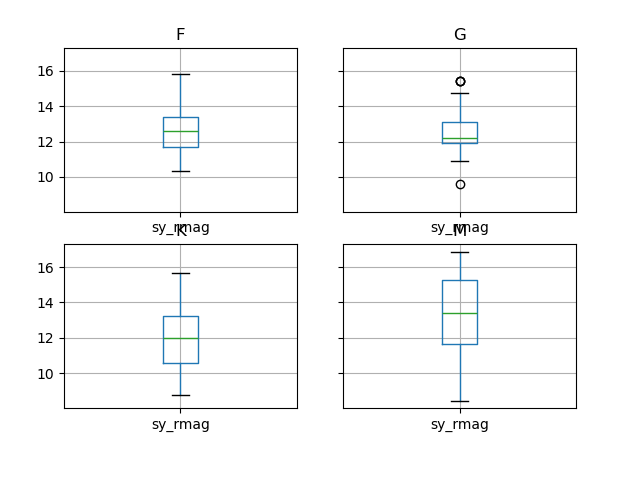
\includegraphics[width=0.9\textwidth,height=\textheight]{../results/figures/sy_rmag.png}

}

\caption{\label{fig-sy-rmag}Box Plot of \texttt{sy\_rmag}}

\end{figure}%

Again, from boxplot Figure~\ref{fig-sy-rmag}, for \emph{M}-class of
stars, the magnitude of the \emph{r}-band is higher than the remaining
classes at 13.4 at the median.

\begin{longtable}[]{@{}
  >{\raggedright\arraybackslash}p{(\columnwidth - 16\tabcolsep) * \real{0.1022}}
  >{\raggedright\arraybackslash}p{(\columnwidth - 16\tabcolsep) * \real{0.0803}}
  >{\raggedright\arraybackslash}p{(\columnwidth - 16\tabcolsep) * \real{0.1460}}
  >{\raggedright\arraybackslash}p{(\columnwidth - 16\tabcolsep) * \real{0.1460}}
  >{\raggedright\arraybackslash}p{(\columnwidth - 16\tabcolsep) * \real{0.0949}}
  >{\raggedright\arraybackslash}p{(\columnwidth - 16\tabcolsep) * \real{0.0949}}
  >{\raggedright\arraybackslash}p{(\columnwidth - 16\tabcolsep) * \real{0.1460}}
  >{\raggedright\arraybackslash}p{(\columnwidth - 16\tabcolsep) * \real{0.0949}}
  >{\raggedright\arraybackslash}p{(\columnwidth - 16\tabcolsep) * \real{0.0949}}@{}}

\caption{\label{tbl-sy-imag}Table of sy\_imag Features}

\tabularnewline

\toprule\noalign{}
\begin{minipage}[b]{\linewidth}\raggedright
Unnamed: 0
\end{minipage} & \begin{minipage}[b]{\linewidth}\raggedright
sy\_imag
\end{minipage} & \begin{minipage}[b]{\linewidth}\raggedright
sy\_imag.1
\end{minipage} & \begin{minipage}[b]{\linewidth}\raggedright
sy\_imag.2
\end{minipage} & \begin{minipage}[b]{\linewidth}\raggedright
sy\_imag.3
\end{minipage} & \begin{minipage}[b]{\linewidth}\raggedright
sy\_imag.4
\end{minipage} & \begin{minipage}[b]{\linewidth}\raggedright
sy\_imag.5
\end{minipage} & \begin{minipage}[b]{\linewidth}\raggedright
sy\_imag.6
\end{minipage} & \begin{minipage}[b]{\linewidth}\raggedright
sy\_imag.7
\end{minipage} \\
\midrule\noalign{}
\endhead
\bottomrule\noalign{}
\endlastfoot
nan & count & mean & std & min & 25\% & 50\% & 75\% & max \\
st\_spectype & nan & nan & nan & nan & nan & nan & nan & nan \\
F & 38.0 & 12.576881578947368 & 1.3087761569920782 & 10.2734 & 11.621 &
12.457899999999999 & 13.171 & 15.4941 \\
G & 102.0 & 12.396317843137258 & 1.1410749290481463 & 9.44522 & 11.6457
& 11.9485 & 12.833225 & 16.6984 \\
K & 112.0 & 11.927328133928572 & 1.5619910548391103 & 8.42724 & 10.4417
& 12.0708 & 13.172 & 14.5213 \\
M & 121.0 & 12.67205818181818 & 2.1675341319081154 & 7.75055 & 10.9702 &
12.9151 & 14.3142 & 17.9112 \\

\end{longtable}

\begin{figure}[H]

\centering{

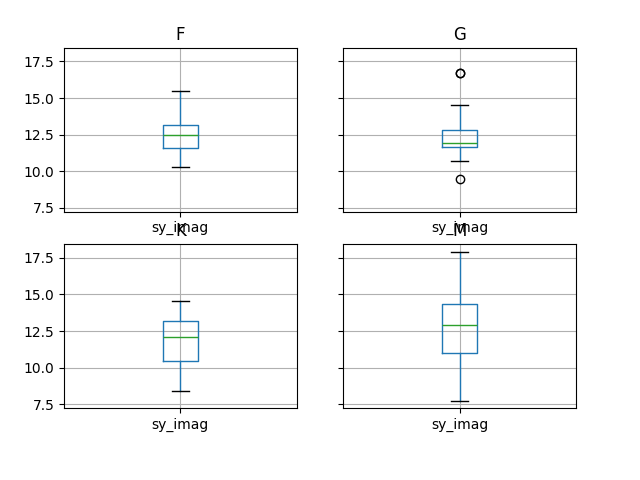
\includegraphics[width=0.9\textwidth,height=\textheight]{../results/figures/sy_imag.png}

}

\caption{\label{fig-sy-imag}Box Plot of \texttt{sy\_imag}}

\end{figure}%

From boxplot Figure~\ref{fig-sy-imag}, for all classes of stars, the
magnitude at the \emph{i}-band is similar.

\begin{longtable}[]{@{}
  >{\raggedright\arraybackslash}p{(\columnwidth - 16\tabcolsep) * \real{0.1022}}
  >{\raggedright\arraybackslash}p{(\columnwidth - 16\tabcolsep) * \real{0.0803}}
  >{\raggedright\arraybackslash}p{(\columnwidth - 16\tabcolsep) * \real{0.1460}}
  >{\raggedright\arraybackslash}p{(\columnwidth - 16\tabcolsep) * \real{0.1460}}
  >{\raggedright\arraybackslash}p{(\columnwidth - 16\tabcolsep) * \real{0.0949}}
  >{\raggedright\arraybackslash}p{(\columnwidth - 16\tabcolsep) * \real{0.0949}}
  >{\raggedright\arraybackslash}p{(\columnwidth - 16\tabcolsep) * \real{0.0949}}
  >{\raggedright\arraybackslash}p{(\columnwidth - 16\tabcolsep) * \real{0.1460}}
  >{\raggedright\arraybackslash}p{(\columnwidth - 16\tabcolsep) * \real{0.0949}}@{}}

\caption{\label{tbl-sy-zmag}Table of sy\_zmag Features}

\tabularnewline

\toprule\noalign{}
\begin{minipage}[b]{\linewidth}\raggedright
Unnamed: 0
\end{minipage} & \begin{minipage}[b]{\linewidth}\raggedright
sy\_zmag
\end{minipage} & \begin{minipage}[b]{\linewidth}\raggedright
sy\_zmag.1
\end{minipage} & \begin{minipage}[b]{\linewidth}\raggedright
sy\_zmag.2
\end{minipage} & \begin{minipage}[b]{\linewidth}\raggedright
sy\_zmag.3
\end{minipage} & \begin{minipage}[b]{\linewidth}\raggedright
sy\_zmag.4
\end{minipage} & \begin{minipage}[b]{\linewidth}\raggedright
sy\_zmag.5
\end{minipage} & \begin{minipage}[b]{\linewidth}\raggedright
sy\_zmag.6
\end{minipage} & \begin{minipage}[b]{\linewidth}\raggedright
sy\_zmag.7
\end{minipage} \\
\midrule\noalign{}
\endhead
\bottomrule\noalign{}
\endlastfoot
nan & count & mean & std & min & 25\% & 50\% & 75\% & max \\
st\_spectype & nan & nan & nan & nan & nan & nan & nan & nan \\
F & 38.0 & 13.088815789473683 & 0.9374631863118148 & 10.4784 & 12.9808 &
13.17575 & 13.463275 & 15.2871 \\
G & 102.0 & 12.9710131372549 & 0.6918843048279733 & 9.60484 & 12.7326 &
13.046 & 13.3566 & 14.4078 \\
K & 112.0 & 11.853661964285717 & 1.5438856430050727 & 7.85169 & 10.6281
& 12.3442 & 13.094574999999999 & 13.9587 \\
M & 121.0 & 12.173695950413222 & 1.659763323241991 & 7.76319 & 11.0226 &
12.7195 & 13.2565 & 15.1016 \\

\end{longtable}

\begin{figure}[H]

\centering{

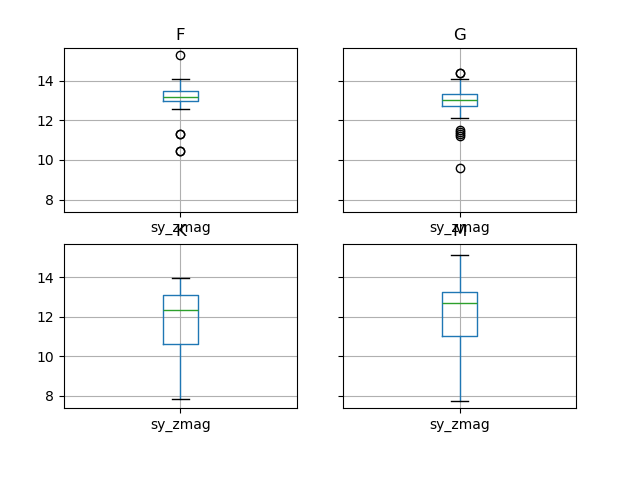
\includegraphics[width=0.9\textwidth,height=\textheight]{../results/figures/sy_zmag.png}

}

\caption{\label{fig-sy-zmag}Box Plot of \texttt{sy\_zmag}}

\end{figure}%

From boxplot Figure~\ref{fig-sy-zmag}, for all classes of stars, the
magnitude at the \emph{z}-band is similar.

\subsection{Classification Analysis}\label{classification-analysis}

\begin{longtable}[]{@{}llllllll@{}}
\toprule\noalign{}
& pl\_name & st\_spectype & sy\_umag & sy\_gmag & sy\_rmag & sy\_imag &
sy\_zmag \\
\midrule\noalign{}
\endhead
\bottomrule\noalign{}
\endlastfoot
count & 373 & 373 & 373.000000 & 373.000000 & 373.000000 & 373.000000 &
373.000000 \\
unique & 219 & 4 & NaN & NaN & NaN & NaN & NaN \\
top & WASP-92 b & M & NaN & NaN & NaN & NaN & NaN \\
freq & 5 & 121 & NaN & NaN & NaN & NaN & NaN \\
mean & NaN & NaN & 16.034040 & 13.802282 & 12.653515 & 12.363340 &
12.388862 \\
std & NaN & NaN & 1.560836 & 1.849799 & 1.735937 & 1.691341 &
1.435804 \\
min & NaN & NaN & 13.093200 & 9.912880 & 8.463130 & 7.750550 &
7.763190 \\
25\% & NaN & NaN & 15.079600 & 12.463100 & 11.650100 & 11.386000 &
11.608400 \\
50\% & NaN & NaN & 15.548300 & 13.664600 & 12.539900 & 12.151500 &
12.839400 \\
75\% & NaN & NaN & 16.479300 & 15.199500 & 13.678000 & 13.425900 &
13.290800 \\
max & NaN & NaN & 21.297500 & 18.729600 & 16.860000 & 17.911200 &
15.287100 \\
\end{longtable}

We can now get an informed description of our cleaned data
Table~\ref{tbl-describe_datset}

\begin{longtable}[]{@{}
  >{\raggedright\arraybackslash}p{(\columnwidth - 12\tabcolsep) * \real{0.1358}}
  >{\raggedright\arraybackslash}p{(\columnwidth - 12\tabcolsep) * \real{0.1852}}
  >{\raggedleft\arraybackslash}p{(\columnwidth - 12\tabcolsep) * \real{0.1358}}
  >{\raggedleft\arraybackslash}p{(\columnwidth - 12\tabcolsep) * \real{0.1358}}
  >{\raggedleft\arraybackslash}p{(\columnwidth - 12\tabcolsep) * \real{0.1358}}
  >{\raggedleft\arraybackslash}p{(\columnwidth - 12\tabcolsep) * \real{0.1358}}
  >{\raggedleft\arraybackslash}p{(\columnwidth - 12\tabcolsep) * \real{0.1358}}@{}}

\caption{\label{tbl-describe\_datset}Table of Dataset Features}

\tabularnewline

\toprule\noalign{}
\begin{minipage}[b]{\linewidth}\raggedright
pl\_name
\end{minipage} & \begin{minipage}[b]{\linewidth}\raggedright
st\_spectype
\end{minipage} & \begin{minipage}[b]{\linewidth}\raggedleft
sy\_umag
\end{minipage} & \begin{minipage}[b]{\linewidth}\raggedleft
sy\_gmag
\end{minipage} & \begin{minipage}[b]{\linewidth}\raggedleft
sy\_rmag
\end{minipage} & \begin{minipage}[b]{\linewidth}\raggedleft
sy\_imag
\end{minipage} & \begin{minipage}[b]{\linewidth}\raggedleft
sy\_zmag
\end{minipage} \\
\midrule\noalign{}
\endhead
\bottomrule\noalign{}
\endlastfoot
373 & 373 & 373 & 373 & 373 & 373 & 373 \\
219 & 4 & nan & nan & nan & nan & nan \\
WASP-92 b & M & nan & nan & nan & nan & nan \\
5 & 121 & nan & nan & nan & nan & nan \\
nan & nan & 16.034 & 13.8023 & 12.6535 & 12.3633 & 12.3889 \\
nan & nan & 1.56084 & 1.8498 & 1.73594 & 1.69134 & 1.4358 \\
nan & nan & 13.0932 & 9.91288 & 8.46313 & 7.75055 & 7.76319 \\
nan & nan & 15.0796 & 12.4631 & 11.6501 & 11.386 & 11.6084 \\
nan & nan & 15.5483 & 13.6646 & 12.5399 & 12.1515 & 12.8394 \\
nan & nan & 16.4793 & 15.1995 & 13.678 & 13.4259 & 13.2908 \\
nan & nan & 21.2975 & 18.7296 & 16.86 & 17.9112 & 15.2871 \\

\end{longtable}

We can now set our y to be the value we are predicting which is
\texttt{spec\_type} and our predictors will be the following features:
\texttt{sy\_umag}, \texttt{sy\_gmag}, \texttt{sy\_rmag},
\texttt{sy\_imag}, \texttt{sy\_zmag}. From this we created a 75\% train
test split to run our data.

\begin{verbatim}
st_spectype
M    0.337165
K    0.295019
G    0.275862
F    0.091954
Name: proportion, dtype: float64
\end{verbatim}

\begin{longtable}[]{@{}r@{}}

\caption{\label{tbl-y-train-test-values}Table of the y Value Counts of
our Train-Test Split}

\tabularnewline

\toprule\noalign{}
proportion \\
\midrule\noalign{}
\endhead
\bottomrule\noalign{}
\endlastfoot
0.337165 \\
0.295019 \\
0.275862 \\
0.091954 \\

\end{longtable}

As seen from Table~\ref{tbl-y-train-test-values} we have a pretty spread
out class with no major class imbalance.

\begin{verbatim}
fit_time       0.003659
score_time     0.000918
test_score     0.674528
train_score    0.721260
dtype: float64
\end{verbatim}

\begin{longtable}[]{@{}lr@{}}

\caption{\label{tbl-lr-cross\_validate}Table of the Cross Validation
Scores from Logistic Regression}

\tabularnewline

\toprule\noalign{}
Unnamed: 0 & 0 \\
\midrule\noalign{}
\endhead
\bottomrule\noalign{}
\endlastfoot
fit\_time & 0.00338473 \\
score\_time & 0.0008708 \\
test\_score & 0.674528 \\
train\_score & 0.72126 \\

\end{longtable}

\subsubsection{Confusion Matrix}\label{confusion-matrix}

One way to get a better understanding of the errors is by looking at how
well the classifier is identifying each class. Which classes are most
frequently confused with each other. Overall accuracy, along with
class-specific metrics like precision, recall, and F1-score for
multi-class classification problems.

It's easier to demonstrate evaluation metrics using an explicit
validation set instead of using cross-validation. So let's create a
validation set as seen below in Table~\ref{tbl-confusion-matrix}.

\begin{longtable}[]{@{}rrrr@{}}

\caption{\label{tbl-confusion-matrix}Table of the Logistic Regression
Confusion Matrix}

\tabularnewline

\toprule\noalign{}
0 & 1 & 2 & 3 \\
\midrule\noalign{}
\endhead
\bottomrule\noalign{}
\endlastfoot
0 & 6 & 0 & 0 \\
0 & 21 & 8 & 0 \\
0 & 2 & 11 & 7 \\
0 & 0 & 2 & 22 \\

\end{longtable}

For better interpretation, we will visualize the confusion matrix
Figure~\ref{fig-cm}.

\begin{figure}[H]

\centering{

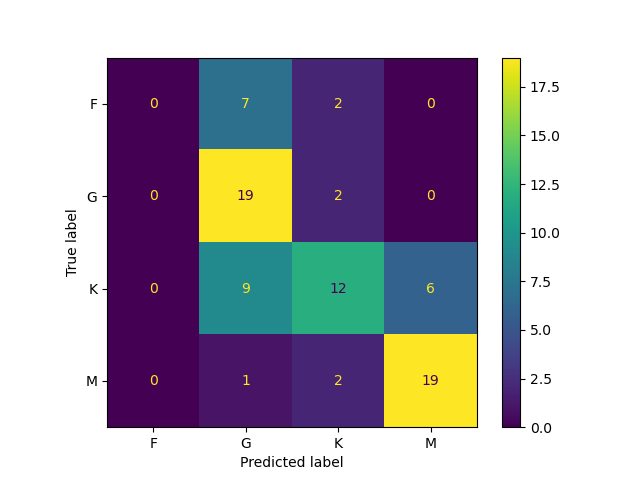
\includegraphics[width=0.9\textwidth,height=\textheight]{../results/figures/confusion_matrix.png}

}

\caption{\label{fig-cm}Visualization of the Confusion Matrix}

\end{figure}%

We can now calculate our accuracy score given by
Table~\ref{tbl-accuracy-score} using our
\texttt{Random\ Forest\ Classifier} given below.

\begin{longtable}[]{@{}rrrr@{}}

\caption{\label{tbl-accuracy-score}Table of Accuracy Score From Random
Forest Classifier}

\tabularnewline

\toprule\noalign{}
0 & 1 & 2 & 3 \\
\midrule\noalign{}
\endhead
\bottomrule\noalign{}
\endlastfoot
0 & 6 & 0 & 0 \\
0 & 21 & 8 & 0 \\
0 & 2 & 11 & 7 \\
0 & 0 & 2 & 22 \\

\end{longtable}

From this we can provide cross validation scores given in
Table~\ref{tbl-rfc-cross-validate} using our
\texttt{Random\ Forest\ Classifier}.

\begin{verbatim}
/home/baron/vanc/DSCI-310-Group-16/venv/dsci/lib/python3.11/site-packages/sklearn/base.py:486: UserWarning: X has feature names, but RandomForestClassifier was fitted without feature names
  warnings.warn(
\end{verbatim}

\begin{verbatim}
Accuracy: 0.29464285714285715
\end{verbatim}

\begin{verbatim}
fit_time       0.175156
score_time     0.005735
test_score     0.827504
train_score    0.987551
dtype: float64
\end{verbatim}

\begin{longtable}[]{@{}lr@{}}

\caption{\label{tbl-rfc-cross-validate}Table of the Cross Validation
Scores from Random Forest Classifier}

\tabularnewline

\toprule\noalign{}
Unnamed: 0 & 0 \\
\midrule\noalign{}
\endhead
\bottomrule\noalign{}
\endlastfoot
fit\_time & 0.00338473 \\
score\_time & 0.0008708 \\
test\_score & 0.674528 \\
train\_score & 0.72126 \\

\end{longtable}

Ultimately from our validation scores, we achieve a much higher test
score from our scaled data with the RandomForestClassifier model of
0.675 compared to LogisticRegression model of 0.675. However our
accuracy score is quite low at 0.

\subsection{Discussion}\label{discussion}

Our model yielded pretty average results with final overall accuracy of
0. This model is not good enough for an automated stellar classification
process. In addition, our model can only classify stars into four
classes due to the limited sample size. However these four classes make
up about 99.8\% of stellar population (Ledrew 2001) so being unable to
classify stars into remaining three classes isn't as big of an issue.
Looking at the confusion matrix, we can see that our model tend to
classify stars as cooler than they actually are (e.g: nine stars were
classified as \emph{G} but were actually \emph{F} class). In order to
improve this model, a larger sample size would help like using the Sloan
Digital Sky Survey dataset instead. Another way to improve the model is
to explore other classification methods such as k nearest neighbours.
Finally, using another photometric system such as UBV could help since
the bands are more seperated resulting in larger difference in
magnitudes between star classes. More research into other classification
methods could most likely yield higher accuracy.

\subsection*{References}\label{references}
\addcontentsline{toc}{subsection}{References}

\phantomsection\label{refs}
\begin{CSLReferences}{1}{0}
\bibitem[\citeproctext]{ref-duan2009automated}
Duan, Fu-Qing, Rong Liu, Ping Guo, Ming-Quan Zhou, and Fu-Chao Wu. 2009.
{``Automated Spectral Classification Using Template Matching.''}
\emph{Research in Astronomy and Astrophysics} 9 (3): 341.

\bibitem[\citeproctext]{ref-hunter2007matplotlib}
Hunter, John D. 2007. {``Matplotlib: A 2D Graphics Environment.''}
\emph{Computing in Science \& Engineering} 9 (03): 90--95.

\bibitem[\citeproctext]{ref-kent1994sloan}
Kent, Stephen M. 1994. {``Sloan Digital Sky Survey.''}
\emph{Astrophysics and Space Science} 217: 27--30.

\bibitem[\citeproctext]{ref-ledrew2001real}
Ledrew, Glenn. 2001. {``The Real Starry Sky.''} \emph{Journal of the
Royal Astronomical Society of Canada, Vol. 95, p. 32} 95: 32.

\bibitem[\citeproctext]{ref-mckinney2010data}
McKinney, Wes et al. 2010. {``Data Structures for Statistical Computing
in Python.''} In \emph{SciPy}, 445:51--56. 1.

\bibitem[\citeproctext]{ref-morgan1942atlas}
Morgan, WW, Philip C Keenan, and Edith Kellman. 1942. {``An Atlas of
Stellar Spectra.''} \emph{University of Chicago}.

\bibitem[\citeproctext]{ref-pedregosa2011scikit}
Pedregosa, Fabian, Gaël Varoquaux, Alexandre Gramfort, Vincent Michel,
Bertrand Thirion, Olivier Grisel, Mathieu Blondel, et al. 2011.
{``Scikit-Learn: Machine Learning in Python.''} \emph{The Journal of
Machine Learning Research} 12: 2825--30.

\bibitem[\citeproctext]{ref-van1995python}
Van Rossum, Guido, and Fred L Drake Jr. 1995. {``Python Tutorial.''}
Centrum voor Wiskunde en Informatica Amsterdam, The Netherlands.

\end{CSLReferences}



\end{document}
